%%% 1206.tex

%% Copyright (C) 2012 LRDE.

%% Permission is granted to copy, distribute and/or modify this document
%% under the terms of the GNU Free Documentation License, Version 1.2
%% or any later version published by the Free Software Foundation;
%% with the Invariant Sections being just ``Copying this document'',
%% no Front-Cover Texts, and no Back-Cover Texts.

%% A copy of the license is provided in the file COPYING.DOC.

\documentclass{techrep} % You can pass the french option if you like.

\usepackage{amsmath, bm}
\usepackage{fancyhdr}
\usepackage{array}
\usepackage{stmaryrd}
\usepackage{graphicx}
\usepackage{gensymb}
\usepackage{vaucanson-g}
\usepackage{amsfonts}
\usepackage{float}
\usepackage{verbatim}
\usepackage{makeidx}
\usepackage[T1]{fontenc}
\usepackage{lmodern}
\usepackage{amsmath}
\usepackage{amsthm}
\usepackage{amsfonts}
\usepackage{tikz}
\usepackage{listings}
\usetikzlibrary{automata,positioning}
\title{SpeakerID - Speaker diarization using Variational Bayes approach}
\author{Victor Lenoir} \revision$LastChangedRevision: 2340 $
\date{June 2012} \email{lenoir@lrde.epita.fr}
%% \www{URL}{TEXT}

\definecolor{dkgreen}{rgb}{0,0.6,0}
\definecolor{gray}{rgb}{0.5,0.5,0.5}
\definecolor{mauve}{rgb}{0.58,0,0.82}

\lstset{ %
  language=Python,                % the language of the code
  basicstyle=\footnotesize,           % the size of the fonts that are used for the code
  numbers=left,                   % where to put the line-numbers
  numberstyle=\tiny\color{gray},  % the style that is used for the line-numbers
  stepnumber=2,                   % the step between two line-numbers. If it's 1, each line
  % will be numbered
  numbersep=5pt,                  % how far the line-numbers are from the code
  backgroundcolor=\color{white},      % choose the background color. You must add \usepackage{color}
  showspaces=false,               % show spaces adding particular underscores
  showstringspaces=false,         % underline spaces within strings
  showtabs=false,                 % show tabs within strings adding particular underscores
  frame=single,                   % adds a frame around the code
  rulecolor=\color{black},        % if not set, the frame-color may be changed on line-breaks within not-black text (e.g. commens (green here))
  tabsize=2,                      % sets default tabsize to 2 spaces
  captionpos=b,                   % sets the caption-position to bottom
  breaklines=true,                % sets automatic line breaking
  breakatwhitespace=false,        % sets if automatic breaks should only happen at whitespace
  title=\lstname,                   % show the filename of files included with \lstinputlisting;
  % also try caption instead of title
  keywordstyle=\color{blue},          % keyword style
  commentstyle=\color{dkgreen},       % comment style
  stringstyle=\color{mauve},         % string literal style
  escapeinside={\%*}{*)},            % if you want to add a comment within your code
  morekeywords={*,...}               % if you want to add more keywords to the set
}

\summary{Speaker diarization and Voice Activity Detection (VAD) play
  an important role in speaker recognition systems, especially in the
  case of multi-speaker signal.\\ We will present speaker diarization
  method based on both Variational Bayes approach (VB) and speaker
  factors. This method has the advantage of using a large number of
  speaker factors as described in state of the art publications on
  speaker recognition systems. To test the performance of this method
  a set of experiments will be done on NIST-SRE 2010 interview data.}

\frenchsummary{La s\'eparation de locuteur et la d\'etection de voix
  jouent un important r\^ole dans les syst\`emes de reconnaissance du
  locuteur, principalement dans le cas d'un signal \`a plusieurs
  locuteurs.\\Nous allons pr\'esenter une m\'ethode de s\'eparation de
  locuteur bas\'ee sur des m\'ethodes variationnelles et sur les
  speaker factors tel que d\'ecrite dans l'\'etat de l'art de
  syst\`emes de reconnaissance du locuteur. Afin de tester les
  performances de cette m\'ethode un ensemble de tests sera effectu\'e
  sur les donn\'ees interview de NIST-SRE 2010.}

\keywords{speaker diarization, factor analysis, speaker recognition,
  gaussian, hidden markov model, gaussian mixture model}

\begin{document}

\section*{Copying this document}
Copyright \copyright{} 2012 LRDE.

Permission is granted to copy, distribute and/or modify this document under
the terms of the GNU Free Documentation License, Version 1.2 or any later
version published by the Free Software Foundation; with the Invariant Sections
being just ``Copying this document'', no Front-Cover Texts, and no Back-Cover
Texts.

A copy of the license is provided in the file COPYING.DOC.

\tableofcontents

\newpage
\chapter{Introduction}

Speaker recognition is a long process. It has multiple problematics
and required pre-processes:
\begin{enumerate}
\item noise filters;
\item features extraction;
\item voice activity detection;
\item speaker diarization.
\end{enumerate}

Speaker diarization is a mandatory step in a speaker recognition
system.  It consists in partitioning an input signal into segments of
different speakers.\\\\ Speaker diarization is a very useful part in
many speech systems, for example in:
\begin{itemize}
\item Speech-to-text followed by a translation of the text, requiring
  speakers identity context
\item Automatic subtitles
\item Pre-processing for speaker recognition/verification
\end{itemize}

In this paper three different speaker diarization (or speaker change
detection) algorithms will be presented: the first one is using hidden
markov model (HMM) and gaussian mixture model (GMM), the second one
proposed by \cite{DIAFACT} is a speaker diarization method based on a
variatonal bayes approach which is a fully probabilistic method using
speaker factors and finally the third one is a streaming system using
HMM and speaker factors.


These three algorithms will be discussed and we'll test the
performance of these methods thanks to a set of experiments on
NIST-SRE 2008 summed data and NIST-SRE 2010 interview data which is a
peculiar data for speaker diarization. Indeed we can have an a priori
on the number of speakers and on the identity of one of the speaker so
it's easier to obtain a segmentation.

In this report only the algorithm using GMM and HMM is using the 2nd
channel of the interview data.

\chapter{Prerequisites}

In this chapter, I will introduce a few notions useful to understand
the algorithms and in which context we use a speaker diarization
algorithm.

\section{Voice Activity Detection}

\subsection{Description}

Voice Activity Detection is a technique used to detect human speech in
an audio recording. The idea is to separate speech segment from
silence and noise. It has a wide application in voice
communication. (used in GSM for example)\\ One of the principal
assumption in VAD algorithms is that the speech is the energetically
dominant signal. VAD has many applications, it's currently used in
hands-free telephony in order to get rid of noise/silence
segments.\\ But also in:
\begin{itemize}
\item Speaker recognition
\item Speech encoding
\item Audio conferencing
\end{itemize}

\subsection{Noise}

Noise can be defined as the contamination of the desired signal by
another unwanted signal.\\ The purpose of the Voice activity detection
is to get rid off the noise and the silent (low-energy) segments.
There are different types of noise, associated with a colour. For
example white noise is a noise with a flat spectrum.

\section{Feature extraction}
\subsection{Cepstral Feature}
In order to detect speech in an audio recording, we have to extract
some features to analyse them. In most of speech recognition's
algorithms, we promote cepstral coefficients unlike raw signal because
the cepstral coefficients have more meanings in speech
recognition.\\ The cepstral coefficients are obtained by doing a
Fourier Transformation. Therefore we have to define a window in order
to process the signal to do a short-term analysis and thus keep a time
data to possibly do the segmentation. (Figure \ref{extractmfcc})\\\\ A
feature vector is extracted for each placement of that window. The Mel
Frequency Cepstral Coefficients (MFCCs Figure
\ref{extractmfccprocess}) are the most important parameters used to
represent speaker vocal track characteristics, they are heuristic
representations of Acoustics propertiesm that simulate the human
ear.\\ In our case the cepstral coefficients are extracted with the
HTKtool HCopy. We use a window of 25ms with a 10ms shift, we extract
the energy and 19 cepstral coefficients, their derivative and their
acceleration. At the end we obtain a sequence of 60-dimensional
cepstral vectors.

\begin{figure}[H]
  \centering
  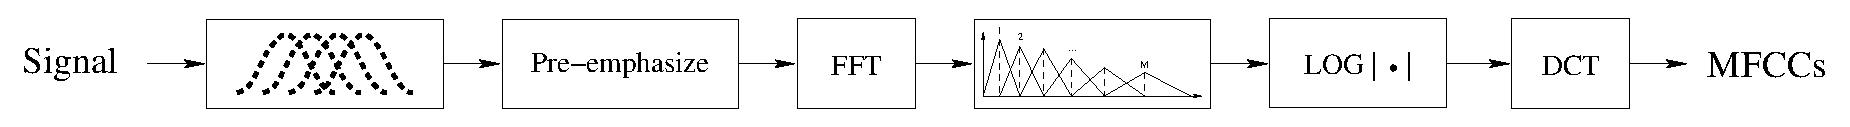
\includegraphics[width=400px]{extract_mfcc_process}
  \caption{Mel-Frequency Cepstral Coefficients extraction process}
  \label{extractmfccprocess}
\end{figure}
\begin{figure}[H]
  \centering 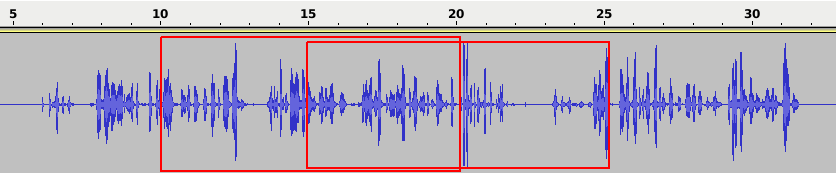
\includegraphics[width=400px]{extract_mfcc}
  \caption{Cepstral coefficients extraction with a window size of 10ms
    and a 5ms shift}
  \label{extractmfcc}
\end{figure}
\subsection{Statistical Feature}
In addition to cepstral coefficients and energy we used other features
which highlight the difference between speech and noise.\\
\begin{center}
  \begin{tabular}{|l|l|l|}
    \hline Feature & Domain & Description\\ \hline Zero Crossing Rate
    & Time & Rate of sign-changes\\ &&along a signal\\ \hline Spectral
    Flatness Measure & Frequency & Coefficient indicating
    the\\ &&flatness of the spectrum\\ \hline Signal Flatness Measure
    & Time & Coefficient indicating the\\ &&flatness of the
    signal\\ \hline
  \end{tabular}
\end{center}
The relevance of each features depend on SNR (Signal to Noise
ratio).\\ Figures \ref{energyplot}, \ref{sfmplot} and
\ref{signalflatness} show the plotting of a few features computed on
an extremely white noised signal. (signal is in blue and feature in
red).\\ We can see that some features are not affected as much as the
others by noise.

\begin{figure}[H]
  \centering 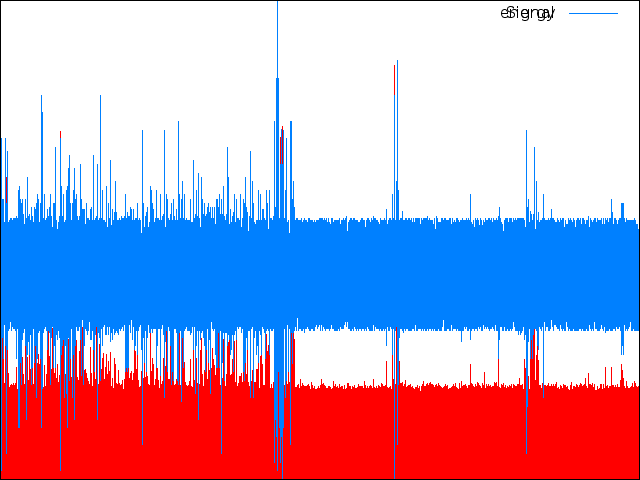
\includegraphics[width=400px, height=100px]{energy_plot}
  \caption{Energy plotting}
  \label{energyplot}
\end{figure}

\begin{figure}[H]
  \centering 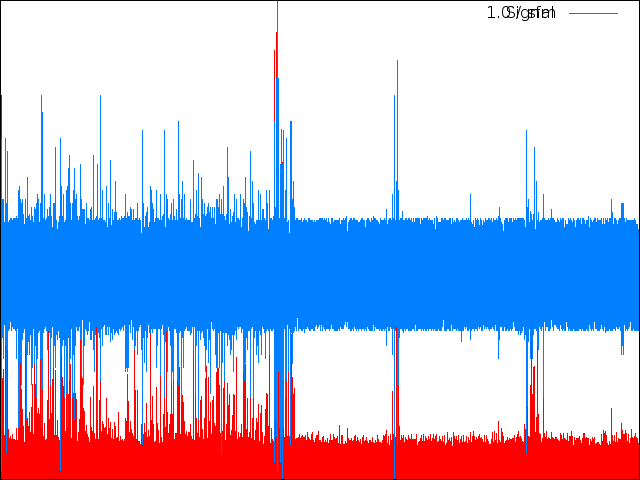
\includegraphics[width=400px, height=100px]{sfm_plot}
  \caption{Inverse of spectral flatness measure plotting}
  \label{sfmplot}
\end{figure}

\begin{figure}[H]
  \centering 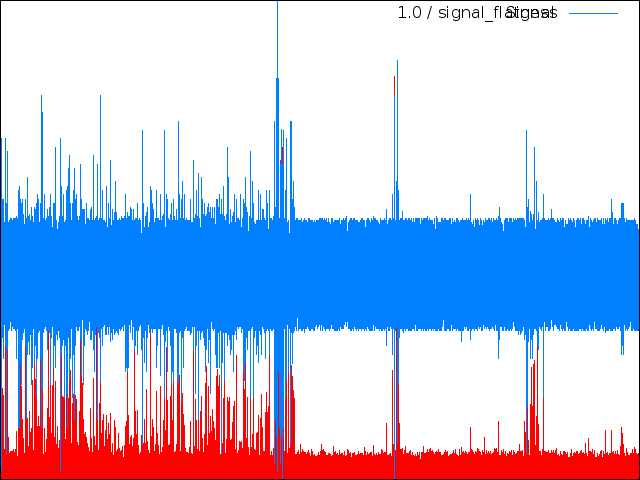
\includegraphics[width=400px,
    height=100px]{signal_flatness}
  \caption{Inverse of signal flatness plotting}
  \label{signalflatness}
\end{figure}

For example we can see that for white noised signal a good feature
would be the inverse of signal flatness (Figure \ref{signalflatness})
because the feature is low when there is white noise and high when
someone is speaking. On the contrary energy (Figure \ref{energyplot})
is affected a lot by the white noised and doesn't cope well with it.

\section{Speaker diarization}
Speaker diarization is the process of partitioning an input speech
file into segments assigned to different speakers. This problem
consists in determining the number of speakers in a given speech file
and in partitioning this speech file into segments.  Most of the time
we determine ths number of speakers in a segment using the Bayesian Information
Criterion (BIC).

In our case, the speaker diarization is done on NIST-SRE10 interview
data which is composed of two channels:
\begin{itemize}
\item Channel 1: The interviewer and the interviewed speaker
\item Channel 2: The interviewer only
\end{itemize}
With these two channels we would like to extract the speech segments
of the speaker interviewed. In this problem the number of speakers is
known, plus we have information on the interviewer identity using the
2nd channel. The purpose of speaker diarization in our case is to
select the segments of the interviewed speaker in the first channel.

A simple solution for this problem would be to process a voice
activity detection algorithm on both channels and then remove the
segments of the 2nd channel from the 1st channel but it obtains bad
result due to an echo of the interviewed speaker on the 2nd channel.

\subsection{Context}

\tikzstyle{cont}=[shape=rectangle,minimum
  size=1.0cm,draw=blue!70,fill=blue!30,font=\small]

\tikzstyle{contred}=[shape=rectangle,minimum
  size=1.0cm,draw=red!70,fill=red!30,font=\small]

  \begin{center}
    \begin{tikzpicture}[scale=0.8,font=\scriptsize]
      \node[cont,initial] (s1) at (0,6) {Audio signal};
      \node[cont] (s2) at (0,4) {Vector of features}
      edge [<-] node[left] {Features extraction} (s1);
      \node[cont] (s3) at (0,2) {Speech features}
      edge [<-] node[left] {VAD} (s2);
      \node[cont] (s4) at (0,0) {Speakers features}
      edge [<-] node[left] {\textcolor{red}{Speaker Diarization}} (s3);
      \node[cont] (s5) at (5,0) {Speaker features}
      edge [<-] node[auto] {Select} (s4);
      \node[cont] (s6) at (5,2) {Speaker Model}
      edge [<-] node[right] {Modeling} (s5);
      \node[cont] (s7) at (5,4) {Score}
      edge [<-] node[right] {} (s6);
      \node (s8) at (5,6) {}
      edge [<-] node[right] {Decision} (s7);
      \node (s8) at (8,4) {Speaker Model}
      edge [->] node[right] {} (s7);
    \end{tikzpicture}
  \end{center}

  In our system:
  \begin{itemize}
    \item Features extraction: 19 MFCCs, energy + their derivatives +
      their accelerations;
    \item Modeling: Estimate Identity-Vector (Ivector) for a speaker
      (600-dim vector which represents the speaker);
    \item Score: Cosine-Distance between 2 Ivectors;
    \item Decision: Threshold the score.
  \end{itemize}  
\chapter{Speaker diarization using HMM/GMM}

In this chapter, I will present a method using Hidden Markov Model
(HMM) and Gaussian Mixture Model (GMM) to solve the speaker
diarization problem. This solution for the speaker diarization problem
is quite simple and works only when the number of speakers is known
and when we can learn 3 GMMs for the: interviewer, interviewed speaker
and noise model.


Its principle is to build a GMM for the noise and a GMM for each of
the two speakers and then do a Viterbi algorithm on a 3 hidden
states-HMM to find the best path/segmentation (the likeliest path).


We then just have to select the interviewed speaker segments found by
the Viterbi algorithm as a solution for our problem.


\section{HMM using GMM}

Hidden Markov Model (HMM) is a widely used statistical Markov model in
speech recognition and signal processing in general. It can modeled
hidden states which generate observations with a certain likelihood
and using the Viterbi algorithm we can retrieve the best sequence of
hidden states which emits the observations.


In our case we have a 3 hidden states HMM (Figure \ref{hmm}):
\begin{itemize}
\item Interviewer state;
\item Interviewed speaker state;
\item Noise/silence state.
\end{itemize}

\tikzstyle{state}=[shape=circle,minimum size=1.7cm,draw=blue!50,fill=blue!20]
\tikzstyle{observation}=[shape=rectangle,minimum size=0.6cm,draw=orange!50,fill=orange!20]
\tikzstyle{lightedge}=[<-,color=red] \tikzstyle{mainstate}=[state,thick]
\tikzstyle{mainedge}=[<-,thick]
\begin{figure}[H]
  \begin{center}
    \begin{tikzpicture}
      % hidden states
      \node[state] (speaker1) at (0,2) {$speaker_1$}
      edge [loop above] node[auto,swap] {$0.9$} ();
      \node[state] (speaker2) at (8,2) {$speaker_2$}
      edge [loop above] node[auto,swap] {$0.9$} ();
      \node[state] (noise) at (4,2) {$noise$}
      edge [<-,bend right=45] node[auto,swap] {$0.1$} (speaker2)
      edge [->,bend left=45] node[auto,swap] {$0.05$} (speaker2)
      edge [<-,bend right=45] node[auto,swap] {$0.1$} (speaker1)
      edge [->,bend left=45] node[auto,swap] {$0.05$} (speaker1)
      edge [loop above] node[auto,swap] {$0.9$} ();
      % observations
      \node[observation] (y1) at (2,0) {$x$}
      edge [lightedge] (speaker1)
      edge [lightedge] (speaker2)
      edge [lightedge] (noise);
      \node[observation] (y2) at (6,0) {$y$}
      edge [lightedge] node[below,pos=0.2] {$0.4$} (speaker1)
      edge [lightedge] (speaker2)
      edge [lightedge] (noise);
    \end{tikzpicture}
  \end{center}
  \label{hmm}
  \caption{An HMM with 3 states which can emit 2 vectors of features $x$ or $y$.}
\end{figure}

In the figure \ref{hmm} the observations $x$ and $y$ are two different
value for the features.

\section{Viterbi algorithm}

The Viterbi algorithm is an algorithm to find the likeliest sequence
of hidden states from a sequence of observations (sequence of features
in our case).


The complexity of this algorithm is: $O(S^2*F)$ where
$S$ is the number of hidden states and $F$ the number of observations.


Generally, the number of hidden states is relatively small compared to the number
of observations so we can approximate this complexity by $O(F)$.

\begin{figure}[H]
  \begin{lstlisting}[frame=single]
    def viterbi(obs, states, start_p, trans_p, emit_p):
    V = [{}]
    path = {}

    for y in states:
    V[0][y] = start_p[y] * emit_p[y][obs[0]]
    path[y] = [y]

    for t in range(1,len(obs)):
    V.append({})
    newpath = {}
    for y in states:
    (prob, state) = max([(V[t-1][y0] * trans_p[y0][y] * emit_p[y][obs[t]], y0) for y0 in states])
    V[t][y] = prob
    newpath[y] = path[state] + [y]
    path = newpath
    (prob, state) = max([(V[len(obs) - 1][y], y) for y in states])
    return (prob, path[state])
  \end{lstlisting}
  \caption{Python-code of the Viterbi algorithm}
  \label{viter}
\end{figure}

\paragraph{Implementation} The implementation of this algorithm was made in C++ so
with a large sequence of observations the probability of the path was
equal to 0 due to precision error. Since we are only interested in
the likeliest path but not its likelihood a workaround would be to
normalize after each observations the previous likelihood.

\section{Gaussian Mixture Model}

Obviously in practice, we don't only have 2 types of possible
observations, we can theoretically have an infinity number of
different observations.

In this case, we have to learn a probability distribution for each of
the hidden state representing the emission probability for a given
observation.

In this work we choose GMMs to represent these distributions.

Gaussian Mixture Model (GMM) is a probabilistic model used to
represent a probability distribution (see Figure \ref{gmmschem} )
defined as below:\\
$$ p(x|\lambda) = \sum_{i=1}^{M} w_i g(x|\mu_i,\Sigma_i)$$
Where\\
$$ g(x|\mu_i,\Sigma_i) =
\frac{1}{(2\pi)^{D/2}|\Sigma_i|^{1/2}}exp{\{-\frac{1}{2}(x-\mu_i)'\Sigma_i^{-1}(x-\mu_i)\}} $$
Where:
\begin{itemize}
\item $wi \ge 0$, $\sum_{i=1}^{M} w_i = 1$;
\item $x$ is the data vector;
\item $\lambda$ is the GMM set of parameters $w_i$, $\mu_i$ and
  $\Sigma_i$ for $1 \leq i \leq M$;
\item $M$ is the number of gaussians component;
\item $w_i$ is the weight of the $i^{th}$ gaussian component;
\item $\mu_i$ is the mean vector of the $i^{th}$ gaussian component;
\item $\Sigma_i$ is the covariance matrice of the $i^{th}$ gaussian
  component;
\item $D$ is the dimension of the $x$ data vector.
\end{itemize}
In order to find the GMM parameters, we use the Linde-Buzo-Gray (LBG)
and the Expectation Maximization algorithm (\cite{EM}). The EM
algorithm is an iterative method for finding maximum likelihood for
given vectors of features.\\ In our case, the $x$ data vector is a
60-dim cepstral feature vector and we use this model to represent the
probability distribution for each of the hidden states of our
HMM.\\ The gaussians we use have diagonal covariance matrix $\Sigma_i$
because it's faster to compute and has less inversibility problem for
the covariance matrix.

\begin{figure}[H]
  \centering 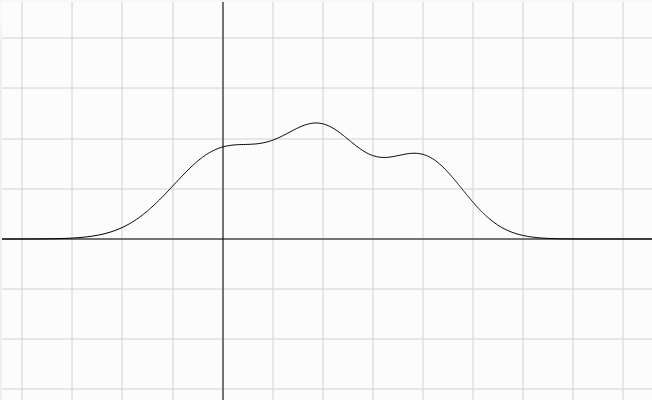
\includegraphics[width=300px]{gmm}
  \caption{Gaussian Mixture Model in 1 dimension with 3 gaussian components.}
  \label{gmmschem}
\end{figure}

\section{Algorithm}

The association of HMM and GMMs (or gaussians) is probably the
most common way to solve a segmentation problem like speaker
diarization, voice activity detection or even speech recognition.  The
tricky part is to learn the 3 GMMs linked to the 3 hidden states.
Fortunately, we do have more data than in a classic speaker
diarization problem:
\begin{itemize}
\item The number of speakers is known;
\item We can have a segmentation of the interviewer thanks to 2nd
  channel.
\end{itemize}
This enable us to find the parameters of the interviewer GMM with the
2nd channel by processing the voice activity detection (VAD) algorithm
described in the paper of \cite{CRIM} in order to remove the
interviewer speech segment from the first channel and then process one more
time the VAD algorithm to find the parameters of the interviewed
speaker GMM and the noise GMM.

Once we've found the GMMs parameters, we only have to set the HMM
parameters: the transition probabilities are fixed as shown in Figure
\ref{hmmgmm} and the emission probabilities are given by the GMMs.

\begin{figure}[H]
  \begin{center}
    \begin{tikzpicture}
      % hidden states
      \node[state] (speaker1) at (0,2) {$speaker_1$}
      edge [loop above] node[auto,swap] {$0.9$} ();
      \node[state] (speaker2) at (8,2) {$speaker_2$}
      edge [loop above] node[auto,swap] {$0.9$} ();
      \node[state] (noise) at (4,2) {$noise$}
      edge [<-,bend right=45] node[auto,swap] {$0.1$} (speaker2)
      edge [->,bend left=45] node[auto,swap] {$0.05$} (speaker2)
      edge [<-,bend right=45] node[auto,swap] {$0.1$} (speaker1)
      edge [->,bend left=45] node[auto,swap] {$0.05$} (speaker1)
      edge [loop above] node[auto,swap] {$0.9$} ();
      % observations
      \node[observation] (y1) at (0,0) {$x$}
      edge [lightedge] node[left,pos=0.8] {$GMM_1(x)$} (speaker1);

      \node[observation] (y2) at (4,0) {$x$}
      edge [lightedge] node[below,pos=0.8] {$GMM_3(x)$} (noise);

      \node[observation] (y3) at (8,0) {$x$}
      edge [lightedge] node[right,pos=0.8] {$GMM_2(x)$} (speaker2);

    \end{tikzpicture}
  \end{center}
  \label{hmmgmm}
  \caption{A HMM with 3 states which can emit with a gaussian probability any possible observation $x$.}
\end{figure}

In our case, an observation is a vector of 60 features: the energy, 19
cepstral coefficients, their derivative and their acceleration.  When
the features are extracted from the channel 1 we only have to process a
Viterbi algorithm on the extracted observations with our HMM to find
the likeliest hidden states path.

We then obtain a segmentation: speaker1/speaker2/noise.

\begin{figure}[H]
  \begin{lstlisting}[frame=single]
    def speaker_diarization(Sound s):
    (GMMinterviewer, GMMuseless, vadseg) = vad(s.channel2)
    (GMMinterviewed, GMMnoise, useless) = vad(sub(s.channel1, vadseg))
    return Viterbi(s.channel1, GMMinterviewer, GMMinterviewed, GMMnoise)
  \end{lstlisting}
  \caption{Python-code of the described algorithm}
  \label{pseudocodehmmgmm}
\end{figure}

The sequence of hidden state will define a segmentation of the
sequence of feature vectors.

\newpage

\section{Output}

\begin{figure}[H]
  \centering 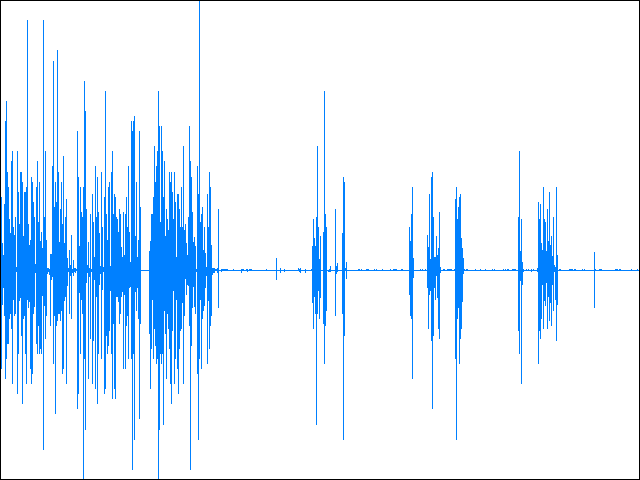
\includegraphics[width=400px,height=100px]{signal_c1}
  \centering 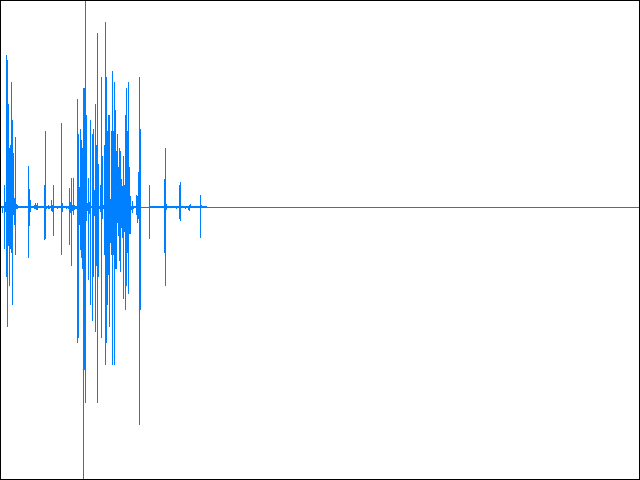
\includegraphics[width=400px,height=100px]{signal_c2}
  \caption{1st and 2nd channel}
  \label{sigc1}
\end{figure}

\begin{figure}[H]
  \centering 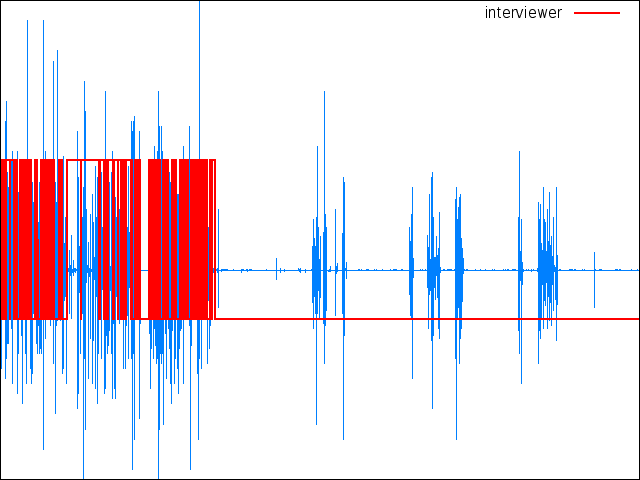
\includegraphics[width=400px,height=100px]{interviewer}
  \centering 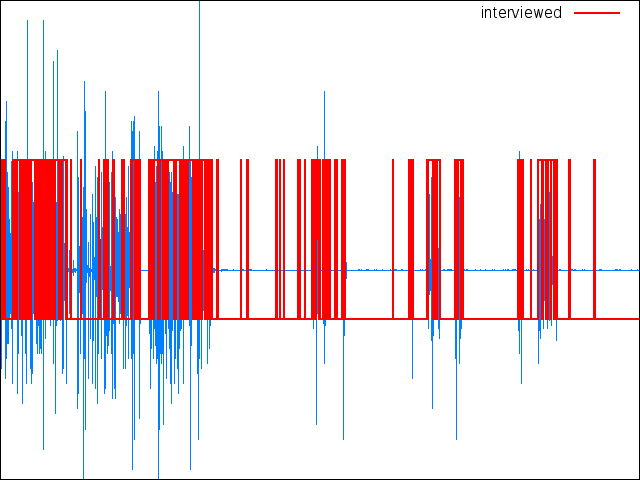
\includegraphics[width=400px,height=100px]{interviewed}
  \caption{Interviewer and Interviewed segmentation of computed from the 1st channel.}
  \label{sigc2}
\end{figure}

It is hard to see if the segmentation of figure \ref{sigc2} is well
done because the two speakers talk at the same time in the beginning
of the signal. This is one of the disadvantage of this algorithm, it
makes hard decision and assigns segment to only one speaker, so if
there is multiple speakers at the same time it will result in a
fragmented segmentation. However we can see that at the end of the signal
the interviewer is not talking which fit to the reality.

\section{Discuss}

\paragraph{Double VAD}
A double VAD consists in applying a VAD on the 2nd channel to obtain
the interviewer speech segments and then remove these segments from
the first channel. We then only have to apply a VAD on the 1st channel
to obtain the final segmentation.

\paragraph{Advantages}
This algorithm is less naive than a double VAD (see Figure
\ref{pseudocodenaive}) and it takes into account both of the identity
of the two speakers during the segmentation while the naive algorithm
doesn't.

\begin{figure}[H]
  \begin{lstlisting}[frame=single]
    def speaker_diarization(Sound s):
    (GMMinterviewer, GMMuseless, vadseg) = vad(s.channel2)
    (GMMinterviewed, GMMnoise, vadf) = vad(sub(s.channel1, vadseg))
    return vadf
  \end{lstlisting}
  \caption{Python-code of a simple version of speaker diarization}
  \label{pseudocodenaive}
\end{figure}

\paragraph{Disadvantages}

This speaker diarization algorithm can only work on the NIST-SRE
interview data since we need to know the number of speakers and the
GMMs parameters for each speakers. The other disadvantages of this
algorithm are the same as the voice activity algorithm used (see paper
of \cite{CRIM}): we make the asumption that there is at least 10\% of
speech in the signal. If there is no speech the procedure will
fail.\\ Furthemore this algorithm can not be applied on-the-fly unless
the parameters of the 3 GMMs are already fixed.\\

\chapter{Speaker diarization using Variational Bayes approach}

In this chapter, I will present the Variational Bayes (VB) approach for
speaker diarization. Furthermore I will quickly introduce one other
speaker diarization algorithm: a streaming system.

These 2 algorithms are presented in the paper of \cite{DIAFACT} and
are both using factor analysis.

For these algorithms a voice activity detection has already been
processed along the signal so there is only remaining speech segments.

\section{Streaming system}

This is the first speaker diarization method which used speaker
factors. The variatonal bayes approach using speaker factors was based
on the this method.

\subsection{Factor analysis}

Factor analysis is a latent variable model closely related to
probabilistic principal component analysis (PPCA) except that the
conditional distribution of the observed data $x$ given the latent
variable $z$ is taken to have a diagonal rather than an isotropic
covariance:
$$p(x|z) = \mathcal{N}(x|Wz + \mu, \Psi)$$

The idea of factor analysis is to find uncorrelated factors from
correlated data. This analysis technique is also a data reduction
technique like PPCA.  

Let $s$ be a randomly chosen speaker dependent supervector (which is
the concatenation of the mean vectors of the speaker GMM), $V$ be a
rectangular matrix with eigenvoices in column, $m$ be the speaker
independent supervector and $y$ be the speaker factors. A common
modeling for speaker recognitions is:

$$ s = m + Vy $$

In most of the speaker recognition systems 300
speaker factors are used. In the streaming system, we are only using
20 speaker factors.

\subsection{Kullback-Leibler divergence}

The Kullback-Leibler divergence is an information divergence criterion
between 2 probability distributions.\\
It is defined as below:
$$D_{KL}(P,Q) = \int_{-\infty}^{\infty}p(x)ln(\frac{p(x)}{q(x)})dx$$
In our case we use the kullback-leibler divergence to match or not 2
speakers modeled by a gaussian distribution.

\subsection{Algorithm}

This technique performs a diarization by slice of about one second
without requiring the following slices, that's why it is called the
streaming system.

Given an audio slice, we extract a stream of 60 features: 19 MFCCs and
energy, their derivative and their acceleration. We then perform a
factor analysis on the whole slice in order to obtain a stream of 20
speaker factors.  To determine the number of speakers talking in the
slice, a Bayesian Information Criterion (BIC) is used.  Once this step
is done we do a clustering of the obtained stream of speaker factors
with the purpose of finding the parameters of the multivariate
gaussians associated to each speakers.

Note that if the number of speakers found by the BIC is 1 we can
directly go the next slice.

Finally we build a Hidden Markov Model (HMM) using the Gaussian for
each state (in our case we consider the number of speakers in a slice
maximized by 2, see Figure \ref{hmmstream}) and we obtain a final
slice segmentation by the Viterbi algorithm.

\begin{figure}[H]
  \begin{center}
    \begin{tikzpicture}
      \node[state] (speaker1) at (0,2) {$speaker_1$}
      edge [loop above] node[auto,swap] {$0.9$} ();
      \node[state] (speaker2) at (4,2) {$speaker_2$}
      edge [loop above] node[auto,swap] {$0.9$} ()
      edge [<-,bend right=45] node[auto,swap] {$0.1$} (speaker1)
      edge [->,bend left=45] node[auto,swap] {$0.1$} (speaker1);

      \node[observation] (y1) at (2,0) {$x$}
      edge [lightedge] node[left,pos=0.05] {$Gauss_1(x)$} (speaker1)
      edge [lightedge] node[right,pos=0.05] {$Gauss_2(x)$} (speaker2);
    \end{tikzpicture}
  \end{center}
  \label{hmmstream}
  \caption{The HMM used in the streaming system.}
\end{figure}

There is still a problem to solve: indeed we have local segmentations
and we can't decide for the moment whether it's the same speakers between
the slices.

To solve this problem we have to define a 256-component GMM for each
of the speakers found in the slices.  At each slice we use the
Kullback-Leibler divergence (information divergence between two
probability distributions) to find the closest speaker model built in
the previous slices.  If the computed divergence is below a threshold
then a new model is built.

\subsection{Discuss}

\paragraph{Advantages} This method has the advantage to be very flexible, there is no a priori about the number of speakers and it's computed dynamically. Moreover it can be applied on-the-fly.

\paragraph{Disadvantages} This method has bad performance relatively to the Variatonal bayes approach. Plus it only uses 20 speaker factors against 300 in the variational bayes approach.

\section{Variational Bayes approach}

Unlike other described methods, this one is fully probabilistic. We
don't make hard decision on a segment.\\ This method required an
Universal Background Model (UBM) which is a huge GMM computed with a
large number of speech files.

\subsection{Variatonal bayesian methods}

In variational inference, the posterior distribution over a set of
unobserved variables $Y$ given some data $X$ (which is the speaker
factors) is approximated by a variational distribution $Q(Y)$ such as:
$$Q(Y) \simeq P(Y|X) $$

In our case the set of unobserved variables is $\{Y,I\}$ where $Y$
specifies the location of speakers in the space of speaker factors and
$I = \{i_1, i_2, ..., i_m\}$ the assignment of segments to speakers:
$i_{ms} = 1$ if speaker $s$ is talking in segment $m$, $i_{ms} = 0$
otherwise.  The segment posteriors is $q_{ms}$ and give the
probability of the segment $m$ to be associated to the speaker $s$\\\\


The idea here is to find a good approximation of the probability of
having a segmentation $I$ given observations $X$: $P(I|X) \simeq Q(I)$
so the diarization solution is given by:
\begin{equation}\label{eq1}
  \arg\max_{I}(P(I|X)) \simeq \arg\max_{I}(Q(I))
\end{equation}

Where we have:
\begin{equation}\label{eq4}
  Q(I) = \prod_{m=1}^{M}Q(i_m)
\end{equation}
and
\begin{equation}\label{eq5}
  Q(i_m) = \prod_{s=1}^{S}q_{ms}^{i_{ms}}
\end{equation}
From \eqref{eq1}, \eqref{eq4} and \eqref{eq5} we obtain:

\begin{equation}\label{eq3}
  \arg\max_{I}(\prod_{m=1}^{M}{\prod_{s=1}^{S}{q_{ms}^{i_{ms}}}})
\end{equation}

Where:
\begin{itemize}
\item $M$ is the number of segments;
\item $S$ is the number of speakers (2 in our case).
\end{itemize}

With one and only one non-zero $i_{ms}$ for each segment $m$.  We can
easily see that this maximization problem can be solved by setting the
$i_{ms}$ associated with the highest $q_{ms}$ probability to 1 so the
lowest probabilities will be set to $1$ ($q_{ms}^0$). Hence the solution for this
diarization problem is for each segment $m$ the speaker talking is
given by:
\begin{equation}\label{eq6}
  \arg\max_{s}(q_{ms})
\end{equation}

The main goal of this algorithm is to find the best approximation for
the segment posterior $q_{ms}$.

\subsubsection{Baum-Welch statistics}

As described by \cite{BAUM} given an observed data $Y$ let
$\gamma_t(c)$ be the posterior probability that the observation at the
time $t$ is generated by UBM mixture component $c$.  For each mixture
component $c$ of the Universal Background Model (UBM) we define the
Baum-Welch statistics as below:
$$N_c = \sum_t{\gamma_t(c)}$$

$$F_c = \sum_t{\gamma_t(c)(Y_t - m_c)}$$

Where:
\begin{itemize}
\item $m_c$ is the mean of the mixture component $c$.
\end{itemize}

\subsection{Algorithm}

\newcommand{\argmax}[1]{\smash{\mathop{{\rm argmax}}\limits_{s}}\, #1}

This method can be summarized as follows:
\begin{enumerate}
\item Extract speaker factors
\item Extract Baum Welch statistics from 1 second segments %need biblio from baum
\item Initialize the segment posteriors randomly
\item For each speaker $s$: synthesize speaker dependent Baum Welch statistics
\item For each speaker $s$: update the speaker posterior
\item For each segment $m$: update the segment posteriors $q_{ms}$ for each
  speaker $s$
\item Iterate step 4-6 until convergence (variations below a defined small $\Delta$)
\item Solution of the segmentation: $\argmax(q_{ms})$ where $q_{ms}$ are the segment posteriors
\end{enumerate}

The steps 2, 4, 5 and 6 will be further detailed.


\subsubsection{Synthesize speaker dependent Baum-Welch statistics}

For each speaker $s$ we synthesize speaker dependent Baum-Welch statistics $N(s)$ and $F(s)$:

$$N(s) = \sum_{m=1}^{M}{q_{ms}N_m}$$
$$F(s) = \sum_{m=1}^{M}{q_{ms}F_m}$$

\subsubsection{Update speaker posterior}
The speaker posterior of $s$ is represented by a normal distribution
of mean $a_s$ and covariance matrix $\Lambda_s^{-1}$:
$$P(Y|X) \simeq Q(Y) = \prod_{s=1}^{S}\mathcal{N}(y_s|a_s,\Lambda_s^{-1})$$

Let $V$ be the eigenvoice of the extracted speaker factors $X$ and
$\Sigma$ be the $CF \times CF$ dimensional covariance matrix whose
diagonal blocs are $\Sigma_1, ..., \Sigma_C$ where $C$ is the number
of components of the UBM, $F$ is the speaker factors dimension and
$\Sigma_i$ is the covariance matrix associated with mixture component
$i$.\\\\ The update formulas for $a_s$ and $\Lambda_s$ are:
$$\Lambda_s = I + V^*\Sigma^{-1}N(s)V$$
$$a_s = \Lambda_s^{-1}V^*\Sigma^{-1}F(s)$$

\subsubsection{Update segment posterior}
Let $\pi_s = \frac{1}{S}$ be the prior probability that a speaker $s$
is talking then for each segment $m$ and speaker $s$ we define
$q_{ms}^{'}$ as below:

$$q_{ms}^{'} = ln(\pi_sP(x_m|a_s)) - \frac{1}{2}tr(V^*N_m\Sigma^{-1}V\Lambda_s^{-1})$$

then the update formula for the segment posteriors is:
$$q_{ms} = \frac{q_{ms}^{'}}{\sum_{s_2=1}^{S}{q_{ms_2}^{'}}}$$%{\sum_{s^'=1}^{S}q_{ms}^{'}}$$
\subsection{Discuss}
\paragraph{Advantages} This method is fully probabilistic and is really effective compared to the other described methods. Plus it uses 300 speaker factors as in speaker recognition state-of-the-art. Moreover the convergence is guaranteed.

\paragraph{Disadvantages} This method required an Universal Background Model while the other methods don't and it cannot be applied on-the-fly.
Furthermore this algorithm alone provides a raw segmentation of 1sec-segments so it requires to resegment using Viterbi.

\chapter{Benchmark}

To compare the Streaming system and the Variatonal Bayes system, a set
of experiments were carried out on the extended trials of the summed
data of the NIST-SRE 2008 by \cite{DIAFACT}.


\paragraph{Diarization Error Rate (DER)} Percentage of miss-classified segments obtained using a reference segmentation provided by NIST.

A comparison of the results using the two speaker diarization
systems is reported in Table \ref{benchou}.\\

\begin{figure}[H]
  \centering
  \begin{tabular}{|l|c|r|}
    \hline
    \textbf{Algorithm} & \textbf{mean DER(\%)} \\
    \hline
    Streaming system & 5.8\\
    \hline
    Streaming system + Viterbi & 4.6\\
    \hline
    Variatonal Bayes & 9.1\\
    \hline
    Variatonal Bayes + Viterbi & 1.9\\
    \hline
  \end{tabular}
  \label{benchou}
  \caption{Benchmark on NIST-SRE 2008 summed data}
\end{figure}

From \ref{benchou}, we can see that the best results are obtained by the variatonal bayes approach with a viterbi re-segmentation in order to avoid 1s-segment.

Note that there is no benchmark for the first HMM/GMM speaker
diarization algorithm because it requires the interview data in order
to work.

\chapter{Conclusion}

Speaker diarization consists in partitioning an input signal into
segments of different speakers.

In this report, we described three different speaker diarization
algorithms: the streaming system which is an on-the-fly speaker
diarization algorithm using speaker factors, the variatonal bayes
approach for speaker diarization which is a fully probabilistic method
also using speaker factors to cluster segments and a speaker
diarization using HMM and GMM only working on NIST interview data
because using the two channels and having an a priori on the number of
speakers.

\paragraph{Achieved work} This report described and discussed the three different speaker diarization methods, from the features extraction to the final segmentation. The speaker diarization using HMM/GMM and the streaming system was implemented and tested on the NIST-SRE 2010 interview data.

\paragraph{Future works} I still have to implement the variatonal bayes approach and the streaming system in order to do a set of experiments on the NIST-SRE 2010 interview data and compare the performance thanks to obtained DET curves.

\bibliography{1206} \nocite{*}

\end{document}

%%% 1206.tex ends here.
